\documentclass{homeworg}
\usepackage{threeparttable}
\usepackage{lscape}
\usepackage{natbib}
\usepackage{amsmath}
\usepackage{graphicx}
\usepackage{listings}
\usepackage{booktabs}
\usepackage{caption}
\usepackage{subcaption}




\title{Bayesian Statistics HW-4}
\author{Weijia Zhao}



\begin{document}
\maketitle

\textbf{Caution} I keep 6 digits for all simulated results. Since it involves random sampling from certain non-degenerative distribution, the results may be slightly different in different trials (and thus from the official solution)

\exercise 
\textbf{Metropolis for Correlation Coefficient} \\
Pairs $(X_i,Y_i)$, $i=1,....,n$ with density $f(x,y|\rho)=\frac{1}{2\pi\sqrt{1-\rho^2}}e^{-\frac{1}{2(1-\rho^2)}(x^2-2\rho xy+y^2)}$, the prior of $\rho$ given by $\pi(\Sigma)=\frac{1}{|\Sigma|^{3/2}}=\frac{1}{(1-\rho^2)^{3/2}}\mathbb{I}(-1\leq \rho \leq 1)$ where 
$\Sigma=\begin{bmatrix}
	1 & \rho \\
	\rho & 1 
\end{bmatrix}$

(a) When $(X_i,Y_i)$ are observed, the likelihood is given by 
\begin{align*}
L(\rho|x_1,x_2,...x_n)&=\Pi_{i=1}^{n}f(x_i,y_i|\rho)\\
&=\Pi_{i=1}^{n}\frac{1}{2\pi\sqrt{1-\rho^2}}e^{-\frac{1}{2(1-\rho^2)}(x_i^2-2\rho x_iy_i+y_i^2)}\\
&=(\frac{1}{2\pi\sqrt{1-\rho^2}})^n e^{-\frac{1}{2(1-\rho^2)}\sum_{i=1}^{n}(x_i^2-2\rho x_iy_i+y_i^2)}
\end{align*}

The posterior distribution is proportional to 
\begin{align*}
\pi(\rho|(x_i,y_i)_{i=1}^n)&\propto L(\theta|x_1,x_2,...x_n)*\pi(\rho)\\
&=(\frac{1}{2\pi\sqrt{1-\rho^2}})^n e^{-\frac{1}{2(1-\rho^2)}\sum_{i=1}^{n}(x_i^2-2\rho x_iy_i+y_i^2)}*\frac{1}{(1-\rho^2)^{3/2}}\mathbb{I}(-1\leq \rho \leq 1) \\
&\propto (1-\rho^2)^{-\frac{n}{2}-\frac{3}{2}}e^{-\frac{1}{2(1-\rho^2)}\sum_{i=1}^{n}(x_i^2-2\rho x_iy_i+y_i^2)} \mathbb{I}(-1\leq \rho \leq 1)
\end{align*}

(b) Assume $n=100$ and the observed pairs $(X_i,Y_i)$ have the summary statistics $\sum_{i=1}^{100}x_i^2=114.9707$,  $\sum_{i=1}^{100} y_i^2=105.9196$ and $\sum_{i=1}^{100}x_iy_i=82.5247$.
The Metropolis algorithm is given by the following steps 
\begin{itemize}
\item Start with an arbitrary initial value $\rho_0$
\item At stage $n$, generate new proposal $\hat{\rho}$ from the uniform distribution $\mathbb{U}(\rho_n-0.1,\rho_n+0.1)$
\item With probability $\theta(\rho_n,\hat{\rho})$\footnote{Note that we flip the notation $\rho$ and $\theta$ compared with the lecture notes since $\rho$ is already taken} we accept the new proposal $\rho_{n+1}=\hat{\rho}$ and with probability $1-\theta(\rho_n,\hat{\rho})$ we reject the new proposal and $\rho_{n+1}=\rho_{n}$
\item Increase n and go to the second step
\end{itemize}
Here in this case the new proposal is from $\mathbb{U}(\rho_n-0.1,\rho_n+0.1)$, thus 
\begin{align*}
q(\hat{\rho}|\rho_n)&=\frac{1}{(\rho_n+0.1)-(\rho_n-0.1)}\mathbb{I}(\rho_n-0.1\leq \hat{\rho}\leq \rho_n+0.1)\\
&=5\mathbb{I}(\rho_n-0.1\leq \hat{\rho}\leq \rho_n+0.1)
\end{align*}
On the other hand, given $\hat{\rho}$, the conditional distribution of $\rho_n$ is $\mathbb{U}(\hat{\rho}-0.1,\hat{\rho}+0.1)$, so $q(\rho_n|\hat{\rho})=5\mathbb{I}(\hat{\rho}-0.1\leq \rho_n\leq \hat{\rho}+0.1)$, thus the acceptance ratio is given by 
\begin{align*}
\theta(\rho_n,\hat{\rho})&=\min(1,\frac{q(\rho_n|\hat{\rho})\pi(\hat{\rho})}{q(\hat{\rho}|\rho_n)\pi(\rho_n)})\\
&=\min(1,\frac{\mathbb{I}(\hat{\rho}-0.1\leq \rho_n\leq \hat{\rho}+0.1)}{\mathbb{I}(\rho_n-0.1\leq \hat{\rho}\leq \rho_n+0.1)}*\frac{(1-\hat{\rho}^2)^{-\frac{n}{2}-\frac{3}{2}}e^{-\frac{1}{2(1-\hat{\rho}^2)}\sum_{i=1}^{n}(x_i^2-2\hat{\rho} x_iy_i+y_i^2)} \mathbb{I}(-1\leq \hat{\rho} \leq 1)}{(1-\rho_n^2)^{-\frac{n}{2}-\frac{3}{2}}e^{-\frac{1}{2(1-\rho_n^2)}\sum_{i=1}^{n}(x_i^2-2\rho_n x_iy_i+y_i^2)} \mathbb{I}(-1\leq \rho_n \leq 1)})\\
&=\min(1,\frac{(1-\hat{\rho}^2)^{-\frac{n}{2}-\frac{3}{2}}e^{-\frac{1}{2(1-\hat{\rho}^2)}\sum_{i=1}^{n}(x_i^2-2\hat{\rho} x_iy_i+y_i^2)} \mathbb{I}(-1\leq \hat{\rho} \leq 1)}{(1-\rho_n^2)^{-\frac{n}{2}-\frac{3}{2}}e^{-\frac{1}{2(1-\rho_n^2)}\sum_{i=1}^{n}(x_i^2-2\rho_n x_iy_i+y_i^2)} \mathbb{I}(-1\leq \rho_n \leq 1)})
\end{align*}

Here notice that $\frac{\mathbb{I}(\hat{\rho}-0.1\leq \rho_n\leq \hat{\rho}+0.1)}{\mathbb{I}(\rho_n-0.1\leq \hat{\rho}\leq \rho_n+0.1)}=1$ and thus cancels, this is because both probability indicates that $|\rho'-\rho_n|\leq 0.1$, this is indeed a symmetric Metropolis. We can then substitute $n=100$ and $\sum_{i=1}^{100}x_i^2=114.9707$,  $\sum_{i=1}^{100} y_i^2=105.9196$ $\sum_{i=1}^{100}x_iy_i=82.5247$ into the expression above

(c) The 
\begin{figure}[h]
	\centering
	\begin{subfigure}[b]{0.48\textwidth}
		\centering
		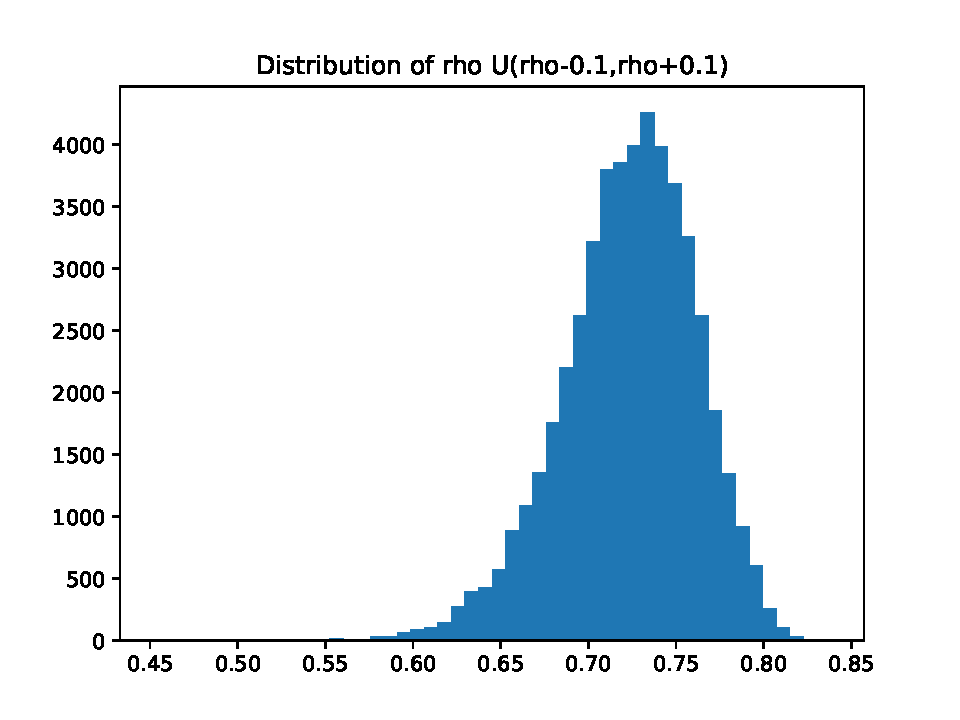
\includegraphics[width=\textwidth]{q1_partc1.pdf}
		\caption{Histogram plot}
	\end{subfigure}
	\hfill
	\begin{subfigure}[b]{0.48\textwidth}
		\centering
		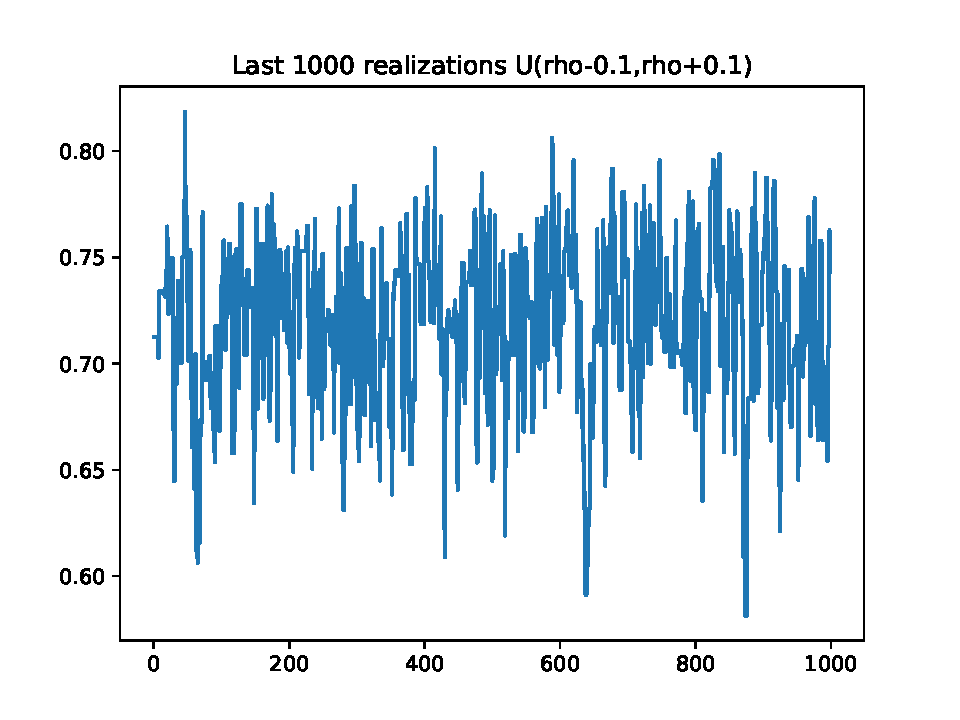
\includegraphics[width=\textwidth]{q1_partc2.pdf}
		\caption{Last 1000 realizations}
	\end{subfigure}
	\caption{Sampling $\rho$ using $\mathbb{U}(\rho_{i-1}-0.1,\rho_{i-1}+0.1)$}
\end{figure}
For Bayes estimator, we just need to calculate the average of simulated $\rho$, which is given by 0.722986 here (This is simulated result, thus may vary a bit in different experiments)

(d)% If we replace the proposal distribution of $\mathbb{U}(\rho_{i-1}-0.1,\rho_{i-1}+0.1)$ by $\mathbb{U}(-1,1)$, then the Metropolis algorithm follows exactly the same steps, but now, 
%\begin{align*}
%q(\hat{\rho}|\rho_{n})&=\frac{1}{1-(-1)} \mathbb{I}(\-1\leq \hat{\rho}\leq 1)\\
%&=\frac{1}{2} \mathbb{I}(\-1\leq \hat{\rho}\leq 1)
%\end{align*}
%Since $\rho_{n}$ and $\hat{\rho}$ are independent, we also have $q(\rho_n|\hat{\rho})=\frac{1}{2} \mathbb{I}(\-1\leq \rho_{n}\leq 1)$. Thus the acceptance ratio is given by 
%\begin{align*}
%\theta(\rho_{n},\hat{\rho})&=\min(1,\frac{q(\rho_n|\hat{\rho})\pi(\hat{\rho})}{q(\hat{\rho}|\rho_n)\pi(\rho_n)})\\
%&=\min(1,\frac{\mathbb{I}(-1\leq \rho_n\leq 1)}{\mathbb{I}(-1\leq \hat{\rho}\leq 1)}*\frac{(1-\hat{\rho}^2)^{-\frac{n}{2}-\frac{3}{2}}e^{-\frac{1}{2(1-\hat{\rho}^2)}\sum_{i=1}^{n}(x_i^2-2\hat{\rho} x_iy_i+y_i^2)} \mathbb{I}(-1\leq \hat{\rho} \leq 1)}{(1-\rho_n^2)^{-\frac{n}{2}-\frac{3}{2}}e^{-\frac{1}{2(1-\rho_n^2)}\sum_{i=1}^{n}(x_i^2-2\rho_n x_iy_i+y_i^2)} \mathbb{I}(-1\leq \rho_n \leq 1)})\\
%&=\min(1,\frac{(1-\hat{\rho}^2)^{-\frac{n}{2}-\frac{3}{2}}e^{-\frac{1}{2(1-\hat{\rho}^2)}\sum_{i=1}^{n}(x_i^2-2\hat{\rho} x_iy_i+y_i^2)} \mathbb{I}(-1\leq \hat{\rho} \leq 1)}{(1-\rho_n^2)^{-\frac{n}{2}-\frac{3}{2}}e^{-\frac{1}{2(1-\rho_n^2)}\sum_{i=1}^{n}(x_i^2-2\rho_n x_iy_i+y_i^2)} \mathbb{I}(-1\leq \rho_n \leq 1)})
%\end{align*}
%It is the same as before as the ratio $\frac{q(\rho_n|\hat{\rho})}{q(\hat{\rho}|\rho_n)}$ is 1 in both cases and thus canceled.
The graphs are shown below and the Bayes estimator can again be obtained by taking the average for simulated $\rho$ and the value is 0.722697 in this case. The histogram graph looks very similar to the previous case (it is a bit more concentrated around the center). The plot for last 1000 realizations looks more different, we see a lot of flat areas, which means the next simulated $\rho$ takes the same value as the last simulated $\rho$, i.e. the new proposal is rejected. Here we can see that under the new regime, the probability of accepting a proposal is lower compared to the previous case
\begin{figure}[h]
	\centering
	\begin{subfigure}[b]{0.48\textwidth}
		\centering
		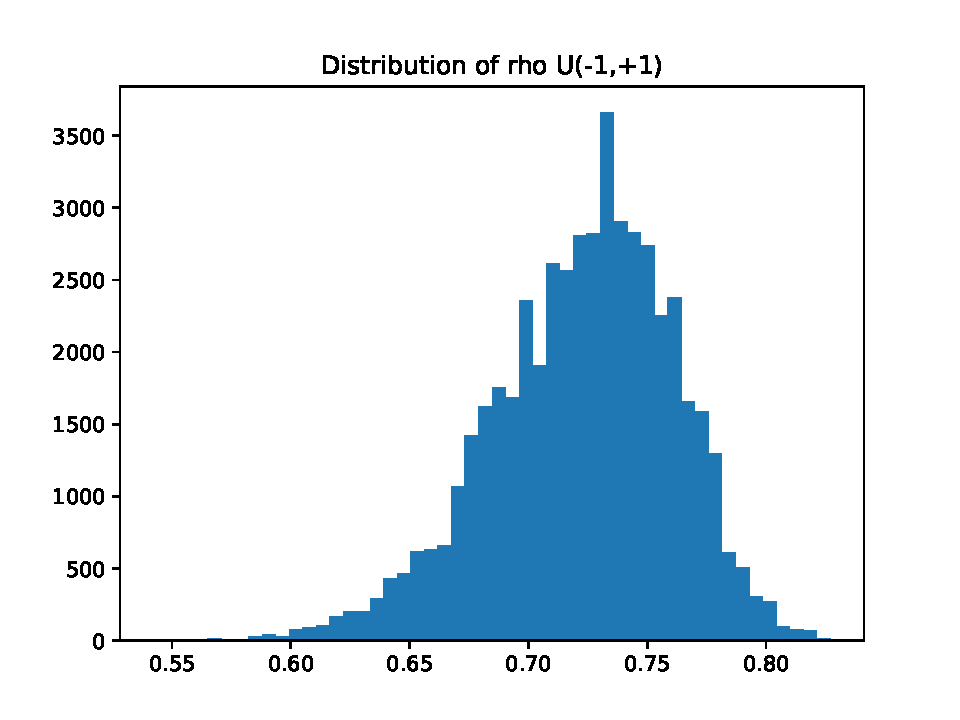
\includegraphics[width=\textwidth]{q1_partd1.pdf}
		\caption{Histogram plot}
	\end{subfigure}
	\hfill
	\begin{subfigure}[b]{0.48\textwidth}
		\centering
		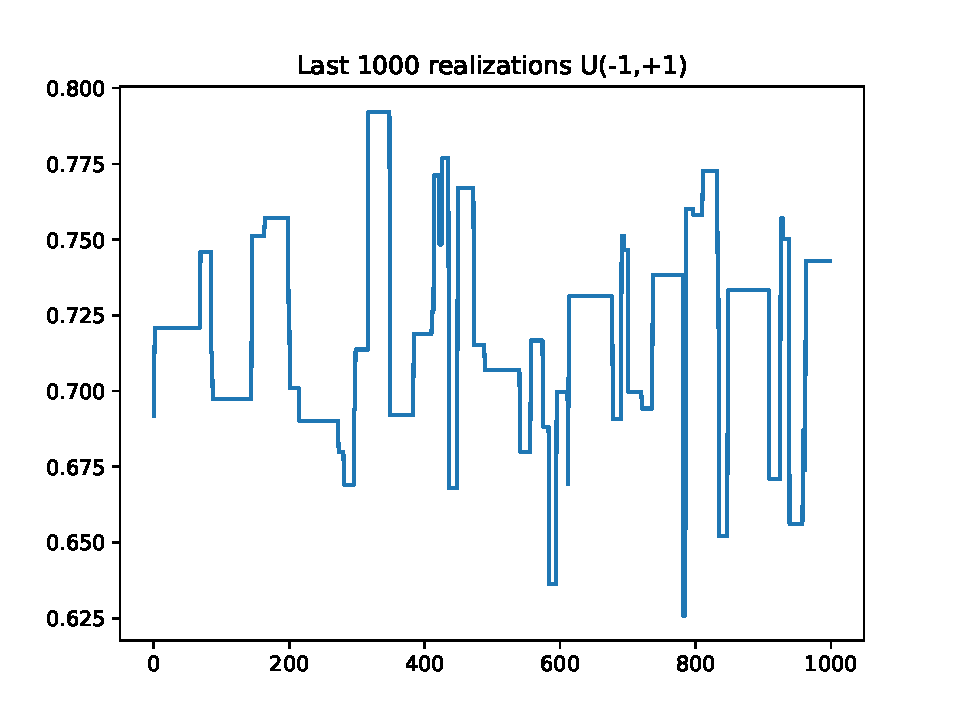
\includegraphics[width=\textwidth]{q1_partd2.pdf}
		\caption{Last 1000 realizations}
	\end{subfigure}
	\caption{Sampling $\rho$ using $\mathbb{U}(-1,+1)$}
\end{figure}


\exercise 
\textbf{Gibbs Sampler and Lifetimes with Multiplicative Frailty} \\
Exponentially distributed lifetime with constant hazard rate $\lambda$. Introduce heterogeneity of hazard with a multiplicative frailty parameter $\mu$, distribution of lifetimes $T_i$ given by 
\begin{align*}
T_i\sim f(t_i|\lambda,\mu)=\lambda\mu e^{-\lambda\mu t_i}, t_i>0,\lambda,\mu>0
\end{align*}
Prior of $(\lambda,\mu)$ $\pi(\lambda,\mu)\propto \lambda^{c-1}\mu^{d-1}e^{-\alpha\lambda-\beta\mu}$, i.e. $\lambda,\mu$ apriori independent with distribution $\Gamma(c,\alpha)$, $\Gamma(d,\beta)$, with $c,d,\alpha,\beta$ known and positive, observe $t_1,t_2,...t_n$

(a) The posterior distribution of $\lambda$ is given by 
\begin{align*}
\pi(\lambda|\mu,{t_i}_{i=1}^n) & \propto \pi(\lambda)*\Pi_{i=1}^{n} f(t_i|\lambda\mu)\\
& =\lambda^{c-1}e^{-\alpha\lambda} \lambda^n \mu^n e^{-\lambda\mu\sum_{i=1}^nt_i}\\
&=\lambda^{n+c-1}\mu^{n} e^{-\lambda(\alpha+\mu\sum_{i=1}^nt_i)} \\
&\propto \lambda^{n+c-1} e^{-\lambda(\alpha+\mu\sum_{i=1}^nt_i)}
\end{align*}
This is the core of a Gamma distribution and we can see $[\lambda|\mu,{t_i}_{i=1}^n]\sim Gamma(n+c,\alpha+\mu\sum_{i=1}^nt_i)$

Similarly, the posterior distribution of $\mu$ is given by 
\begin{align*}
\pi(\mu|\lambda,{t_i}_{i=1}^n) & \propto \pi(\mu)*\Pi_{i=1}^{n} f(t_i|\lambda\mu)\\
& =\mu^{d-1}e^{-\beta\mu} \lambda^n \mu^n e^{-\lambda\mu\sum_{i=1}^nt_i}\\
&=\mu^{n+d-1}\lambda^{n} e^{-\mu(\beta+\lambda\sum_{i=1}^nt_i)} \\
&\propto \mu^{n+d-1} e^{-\mu(\beta+\lambda\sum_{i=1}^nt_i)} 
\end{align*}
This is also the core of a Gamma distribution and we can see that $[\mu|\lambda,{t_i}_{i=1}^n]\sim Gamma(n+d,\beta+\lambda\sum_{i=1}^nt_i)$

(b) The Gibbs sampler follows the following several steps
\begin{itemize}
\item Start with $\mu=0.1$
\item Sample $\lambda'\sim Gamma(n+c,\alpha+\mu\sum_{i=1}^nt_i)$, set $\lambda=\lambda'$
\item Sample $\mu'\sim Gamma(n+d,\beta+\lambda\sum_{i=1}^nt_i)$, set $\mu=\mu'$
\item With the newly obtained $\mu$ and $\lambda$, got back to step (2) and repeat until we get enough observations (ignore the first 1000 observations)
\end{itemize}

(c) The graphs are shown below. Note that we remove one more observation from the series of $\mu$ since it has one more initial value compared with the series of $\lambda$. The posterior mean of $\mu$ is given by  0.695968
 and posterior mean of $\lambda$ is given by 0.054395. The posterior variance of $\mu$ is given by 0.066731 and posterior variance of $\lambda$ is given by 0.000361.  The 95\% equitailed credible set (calculated by percentile of the simulated values) for $\mu$ is (0.316929, 1.311192) and the 95\% equitailed credible set for $\lambda$ is (0.025294, 0.098936) (These are simulated results, thus may vary a bit in different experiments)


\begin{figure}[h]
	\centering
	\begin{subfigure}[b]{0.52\textwidth}
		\centering
		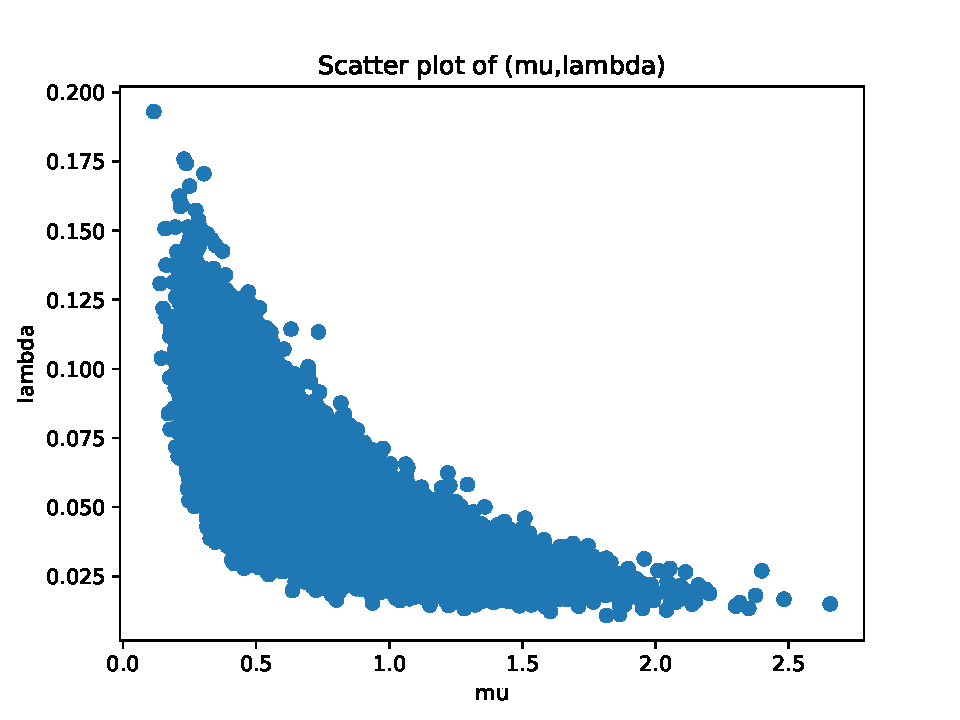
\includegraphics[width=\textwidth]{q2_partc_scatter.pdf}
		\caption{Histogram plot}
	\end{subfigure}
	\hfill
	\begin{subfigure}[b]{0.48\textwidth}
		\centering
		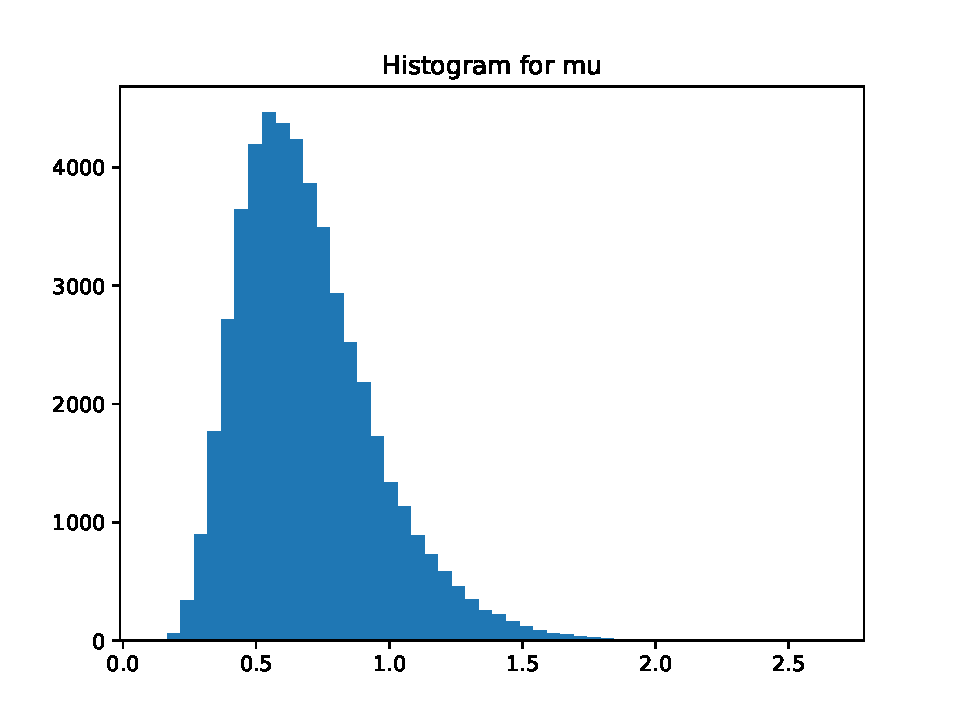
\includegraphics[width=\textwidth]{q2_partc_hist_mu.pdf}
		\caption{Histogram for $\mu$}
	\end{subfigure}
	\begin{subfigure}[b]{0.48\textwidth}
	\centering
	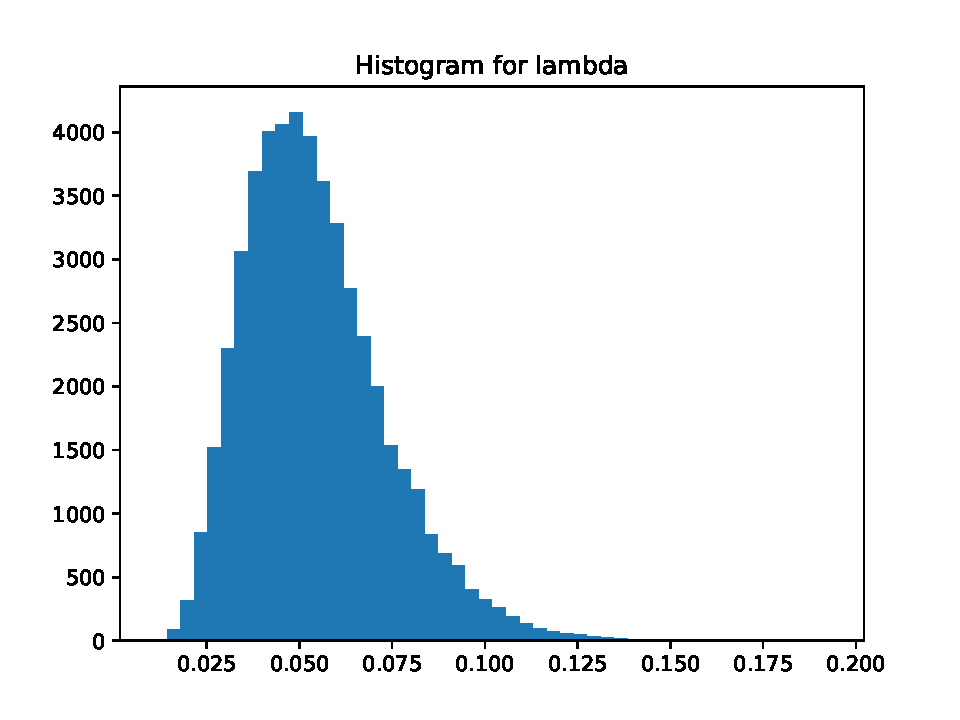
\includegraphics[width=\textwidth]{q2_partc_hist_lambda.pdf}
	\caption{Histogram for $\lambda$}
\end{subfigure}
	\caption{Gibbs Sampling}
\end{figure}

(d) Bayes estimator of the product is given by $\frac{1}{50000}\sum_{i=1}^{50000}\lambda_i*\mu_i=0.034253$ (This is simulated result, thus may vary a bit in different experiments)
%\setlength\bibsep{0pt}
%\bibliographystyle{apalike}
%\bibliography{hw1}

\newpage
\textbf{Code for Q1}
\lstinputlisting[language=Python]{q1.py}

\newpage
\textbf{Code for Q2}
\lstinputlisting[language=Python]{q2.py}
%\lstinputlisting[]{Untitled.do}

\end{document}








